% Kapitel 2 mit den entsprechenden Unterkapiteln
% Die Unterkapitel können auch in separaten Dateien stehen,
% die dann mit dem \include-Befehl eingebunden werden.
%-------------------------------------------------------------------------------
\chapter{Analyse der Produktfunktionen}

%Die Kapitel müssen mit Inhalt gefüllt werden!. Eine Bereiche habe ich beuwsst schon bei der Verteildung der Diagramme zusammengefasst 
%In diesen Bereichen möchte ich euch bitten die jeweiligen Unterpunkte kurz mit den Oberpunkten zu vergleichen und zu argumentieren 
%warum es sich um triviale Spezialfälle handelt die keiner näheren beschreibung bedürfen
%
% Ich hab mal immer davon geschrieben welche Bereich von wem gemacht werden

\section{Analyse der Funktionalität /F100/: Spezifikation einlesen}
Das Einlesen einer Spezifikation aus einem vom Nutzer angegebenen Dateipfad
gliedert sich in mehrere Teilfunktionalutäten. Zunächst muss der Anwender den
Dateipfad auswählen. Dafür sollte ein Datei-Dialog zum Einsatz kommen.
Danach muss die ausgewählte Datei geöffnet, geprüft und geparst werden. Für
diese Aufgaben bietet sich eine spezialisierte Komponente an, um alle
Eigenheiten des Dateiformates von der Oberfläche und dem Simulator abzukapseln.
Der ausgelesene Datensatz nun zum Starten einer neuen Simulation verwendet,
dafür muss eine eventuell laufende Simulation beendet werden. Es bietet sich
an, diese Funktionen als Schnittstelle zu kapseln und die konkrete Implementierung
der Simulator-Komponente zu überlassen.

\begin{figure}
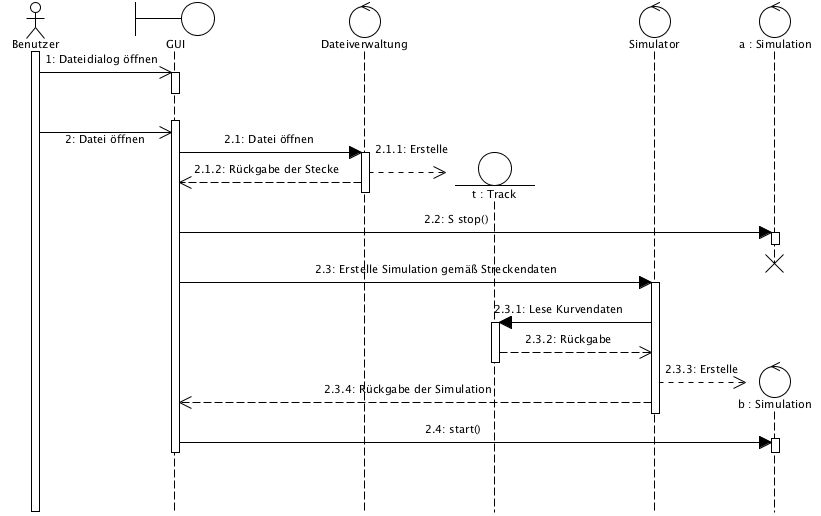
\includegraphics[width=16cm]{bilder/spezifikation_einlesen}
\caption{Sequenzdiagramm für \textit{Spezifikation einlesen}}
\end{figure}

%Christian/Matthias

%kann man dies ggf Q40 zuordnen?
\section{Analyse von Funktionalität :  Renderloop}
Da es sich um ein System handelt, indem eine ständige Berechnung (Loop) zur Laufzeit notwendig wird, einerseits durch die 3D-Anzeige die eine ständige aktualisierung erwartet und andererseits durch
die Simulation an sich, ist es sinnig diesen Vorgang ebenfalls näher zu beleuchten.

\begin{figure}
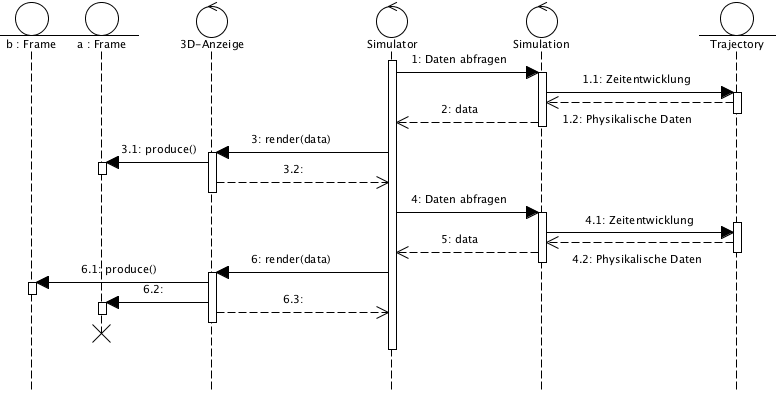
\includegraphics[width=16cm]{bilder/render_loop}
\caption{Sequenzdiagramm für \textit{Renderloop}}
\label{labelname}
\end{figure}
%Simon:
\section{Analyse von Funktionalität /F200/ :  Starten/Stoppen der Simulation}
Der Anwender kann über die 2D GUI die Simulation starten. Dabei wird die Information an die Render Loop weitergeleitet, die die das 3D Bild anzeigt, das HUD anzeigt, die Bahnberechnung startet und die Aufzeichnung startet. 
Der Anwender kann außerdem über die 2D GUI die Simulation stoppen. Dabei wird die Information an die Render Loop weitergeleitet, die zuerst die Aufzeichnung beendet und speichert, danach die Bahnberechnung anhält, dann das HUD ausbledent und zum Schluss das 3D Bild ausblendet.
\begin{figure}
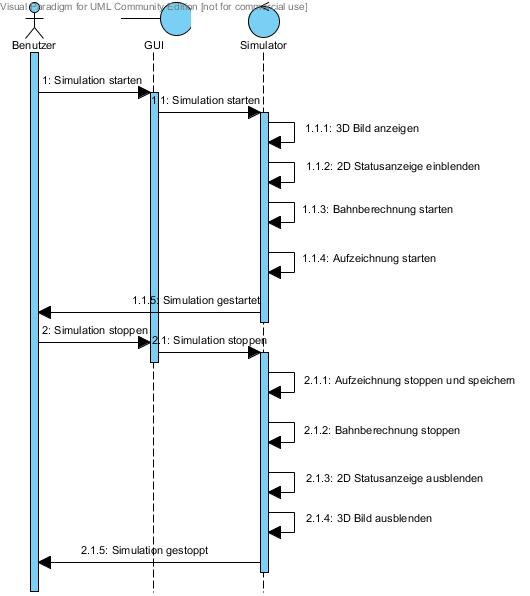
\includegraphics[width=16cm]{bilder/Simulator_Starten_Stoppen}
\caption{Sequenzdiagramm für das \textit{Starten und Stoppen der Simulation}}
\label{labelname}
\end{figure}
%Robin
\section{Analyse von Funktionalität /F300/ :  Pausieren der Simulation}
Der Anwender hat während der Simulation die Möglichkeit diese anzuhalten und sie später fortzusetzen, ohne dass die Pausierung Auswirkungen auf das Simulationsergebnis hat.
\begin{figure}
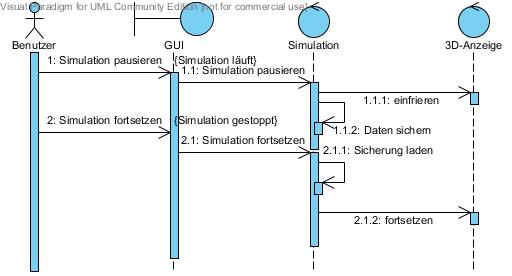
\includegraphics[width=\linewidth]{bilder/Pausieren.jpg}
\caption{Sequenzdiagramm für \textit{Pausieren der Simulation}}
\label{labelname}
\end{figure}

%Daniel
\section{Analyse von Funktionalität /F400o/ :  Video aufzeichnen}
Der Anwender kann über die GUI die Eingabe tätigen ein Video aufzeichnen zu wollen, sofern nicht gerade eine Aufnahme läuft. Die GUI gibt diese Anweisung an die 3D-Anzeige weiter, die nun mit der
Videoaufnahme beginnt. Dies geschieht so lange, bis der Anwender die Videoaufzeichnung stoppt. In diesem Fall wird die Aufzeichnung angehalten und die Videodatei wird gespeichert.


\begin{figure}
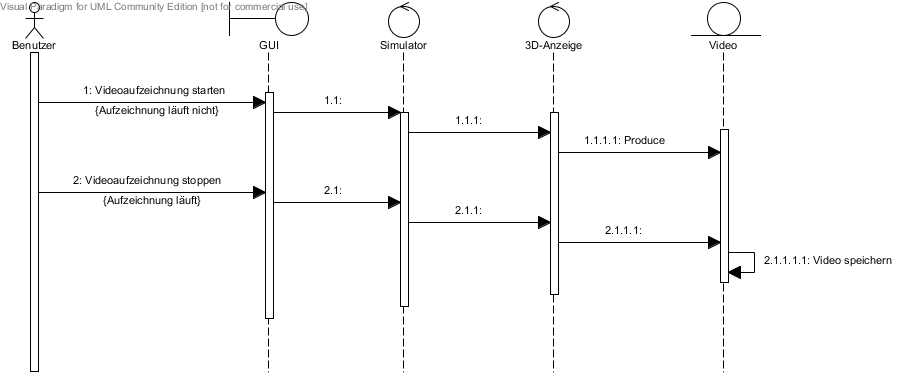
\includegraphics[width=16cm]{bilder/Video_aufzeichnen}
\caption{Sequenzdiagramm für \textit{Video aufzeichnen}}
\label{labelname}
\end{figure}

%Matthias/Christian
\section{Analyse von Funktionalität /F500/ :  Einstellungen ändern}
\subsection{Analyse von Funktionalität /F510o/ :  Physikalische Paramter anpassen}
% Hier reicht ein Sequenzdiagramm, das zeigt das Änderungen an den physikalischen Paramtern das stoppen der Simulation zur Folge haben
% die folgenden Kapitel würde ich daher in einem zusätzlichen Textkommentar zusammenfassen
\subsubsection{Analyse von Funktionalität /F511o/ :  Gravitation anpassen}
\subsubsection{Analyse von Funktionalität /F512o/ :  Wagenmasse anpassen}
%Matthias
\subsection{Analyse von Funktionalität /F520/ :  Simulationsparameter ändern}
Die Veränderung von Parametern die die Simulation direkt betreffen fallen unter diese Oberklasse. Die einzelnen Unterpunkte werden in den 2 folgenden Kapiteln erläutert. Im wesentlichen Fallen hier 
auch einfache Veränderungen an, die als atomistisch und somit unkritisch anzusehen sind. In der Folge werden diese Use-Cases nicht extra in Sequenzdiagrammen abgebildet.
\subsubsection{Analyse von Funktionalität /F521o/ :  Dekorative Umgebung anpassen}
Da diese Aktion in den Datenbestand des 3D-Kontext eingreift gibt es einen interessanten Fall in dem das direkte Setzen der Deko nicht möglich ist. 
Der User fordert die Veränderung der Deko über die 2D-GUI an (2). Kurz zuvor wurde aber das Render eine Frames(1) angefordert. In der Folge muss die 3D Anzeige mit der Veränderung der Konfiguration (1.3)
bis zum Abschluss des Rendervorgangs (1.2) warten. Dann kann die Deko gemäß der Uservorgaben geladen werden(1.4). In (1.5) meldet sich die 3D-Anzeige bei den anderen Komponenten zurück. 

\begin{figure}
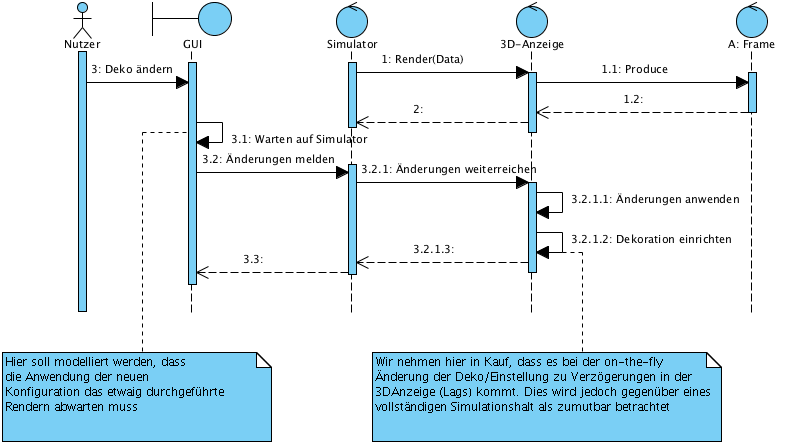
\includegraphics[width=16cm]{bilder/change_graphic_deko}
\caption{Sequenzdiagramm für \textit{Dekorative Umgebung anpassen}}
\label{labelname}
\end{figure}
Es wird hier in Kauf genommen, dass die Simulation für eine spürbare Zeit unterbrochen wird um die Deko zu laden. Dies wird als zumutbar angenommen um undefinierte Zustände zu verhindern. 
Außerdem wird erwartet, dass die Funktionalität selten während der laufenden Simulation sondern vor dem Start genutzt wird wo auch Wartezeiten akzeptabel sind.

\subsubsection{Analyse von Funktionalität /F522o/ :  Simulatioszeit anpassen}
Die Simulationsgeschwindigkeit wird, aufgrund der Implementierung eines numerischen Lösungsverfahrens für die Berechnung der Daten ein diskreter Zeitschritt sein. Dieser Wert kann direkt und entsprechend
den Anforderungen des Nutzers gesetzt werden. Das einfache Durchreichen über die GUI an den Simulator wird nicht in einem zusätzlichen Sequenzdiagramm dargestellt.
%Matthias
\subsection{Analyse von Funktionalität /F530/ :  Graphische Einstellungen ändern}
Die Anpassung der grafischen Einstellung bezieht sich hier zunächst allgemein auf graphische Einstellungen. Besonders interessant ist dabei jedoch der Fall der Veränderung von Einstellungen die 
die 3D-Anzeige betreffen. 

\begin{figure}
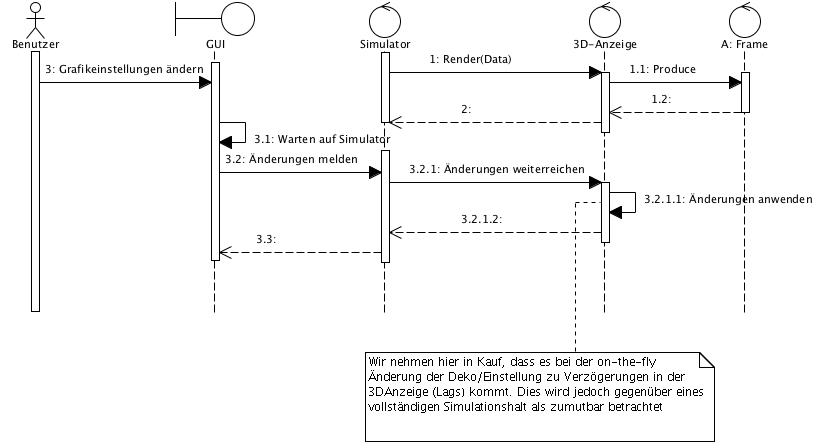
\includegraphics[width=16cm]{bilder/change_graphic_config}
\caption{Sequenzdiagramm für \textit{Graphische Einstellungen ändern}}
\label{labelname}
\end{figure}
Fordert der Nutzer die Veränderung von Einstellungen aus dem 3D-Kontext an (2), so besteht die Möglichkeit, dass zum gleichen Zeitpunkt ein Frame, initiiert durch den Simulator (1), gerendert wird. 
Die GUI (hier für den 2D-Anteil) wird die Anfrage des Benutzer an die 3D-komponente weiterreichen(2.1) und eine etwaige Bestätigung (beispielsweise durch Statusveränderung des Konfigurationsdialogs) an den 
User ausgeben (2.2). Die 3D-Komponente muss jetzt den Renderprozess abwarten und darf erst dann die veränderte Konfiguration anwenden um ungültige Zustände zu vermeiden. Die Anwendung der Konfiguration verzögert 
die Rückmeldung der Bereitschaft an den Simulator(2.1.4) um sicherzustellen, dass nicht mit einem neuen Frame begonnen wird bevor die Einstellungen übernommen wurden. 

Bei diesem Vorgehen wird in Kauf genommen, dass es für das Frame was auf die Einstellungsänderung folgt zu einer Verzögerung in der Darstellung kommt. Dies muss jedoch als zumutbar erachtet werden, da zum einen
eine Zeitdauer im Millisekundenbereich zu erwartet ist. Die Alternativen beinhalten wesentlich störendere Artefakte oder aber das grundsätzliche Anhalten der Simulation nach Änderungen an den Einstellungen.

%Daniel
\subsection{Analyse von Funktionalität /F531/ :   Neuanordnung (Interface)}
Der Anwender hat die Möglichkeit die Segmente innerhalb der GUI nach seinen eigenen Bedürfnissen einzurichten. Um dies zu tun, muss er nur die Eingabe in der GUI tätigen, die Segmente entsperren zu wollen.
Nun sind sie so lange frei positionierbar, bis er die Eingabe tätigt sie wieder sperren zu wollen.
\begin{figure}
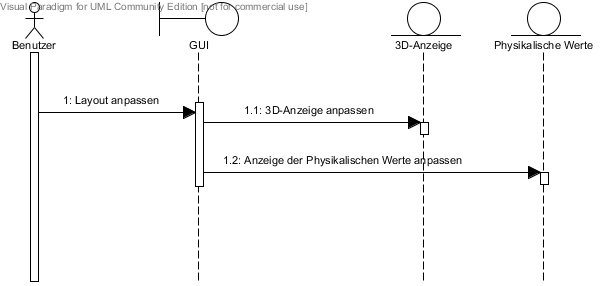
\includegraphics[width=16cm]{bilder/Interface_Neuanordnung}
\caption{Sequenzdiagramm für \textit{Neuanordnung (Interface)}}
\label{labelname}
\end{figure}
%Simon
\subsubsection{Analyse von Funktionalität /F532/ :  Ein-/Ausblenden von Beschleunigungsdaten}
Der Anwender hat die Möglichkeit, sich die Beschleunigungsdaten anzeigen zu lassen. Dabei werden die Daten berechnet und an das HUD übergeben, dass die Beschleunigung dann anzeigt. Zusätzlich hat der Anwender die Möglichkeit die Beschleunigungsdaten wieder auszublenden. Dabei wird die Darstellung der Beschleunigungsdatei geschlossen.
\begin{figure}
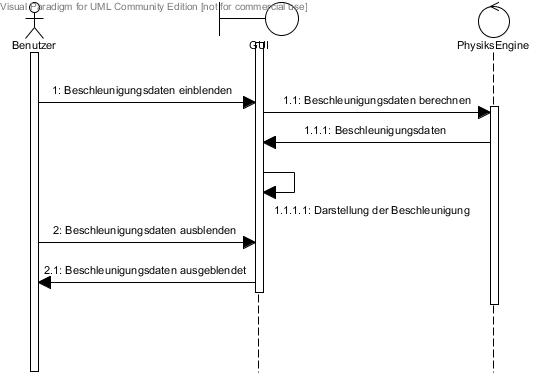
\includegraphics[width=16cm]{bilder/Simulator_Beschleunigung}
\caption{Sequenzdiagramm für \textit{Ein-/Ausblenden von Beschleunigunsdaten}}
\label{labelname}
\end{figure}
%Robin
\subsubsection{Analyse von Funktionalität /F533o/ :  Kameraperspektive ändern}
Während der Simulation kann der Anwender die Perspektive der Kamera ändern, ohne dass dabei die Simulation unterbrochen wird. Um einen unterbrechungsfreien Ablauf zu erreichen, errechnet die Simulation zum nächstmöglichen Zeitpunkt die gewählte Kameraeinstellung und stellt sie ab diesem Zeitpunkt dar. 
\begin{figure}
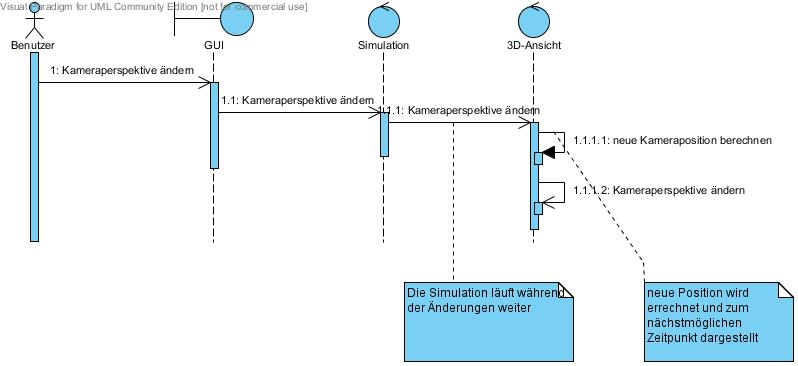
\includegraphics[width=\linewidth]{bilder/Kameraperspektive.jpg}
\caption{Änderung der Kameraperspektive}
\label{Kameraperspektive}
\end{figure}
%Konstantin
\section{Analyse von Funktionalität /F1000/ :  Warnung vor hoher Beschleunigung}
%Marco:
\section{Analyse von Funktionalität /F1100/ :  Erkennung von Veränderungen an der Ursprungsdatei}
